\newcounter{descriptcounti}
\newcounter{descriptcountii}
\newlist{enumfunctional}{description}{2}
\setlist[enumfunctional,1]{%
  before={\setcounter{descriptcounti}{0}%
          \renewcommand*\thedescriptcounti{\myprefix\arabic{descriptcounti}}}
  ,font=\bfseries\stepcounter{descriptcounti}\thedescriptcounti~
}
\setlist[enumfunctional,2]{%
  before={\setcounter{descriptcountii}{0}%
          \renewcommand*\thedescriptcountii{\myprefix\arabic{descriptcounti}.\arabic{descriptcountii}}}
  ,font=\bfseries\stepcounter{descriptcountii}\thedescriptcountii~
}

\newlist{enumnonum}{description}{1}
\setlist[enumnonum,1]{%
  before={\setcounter{descriptcounti}{0}%
          \renewcommand*\thedescriptcounti{\myprefix}}
  ,font=\bfseries\stepcounter{descriptcounti}\thedescriptcounti
}

% Do not forget to include Introduction
%---------------------------------------------------------------
% \chapter{Introduction}
% uncomment the following line to create an unnumbered chapter
\chapter*{Introduction}\addcontentsline{toc}{chapter}{Introduction}\markboth{Introduction}{Introduction}
%---------------------------------------------------------------
\setcounter{page}{1}

% The following environment can be used as a mini-introduction for a chapter. Use that any way it pleases you (or comment


%---------------------------------------------------------------
\section{Podkapitola}
%---------------------------------------------------------------


%---------------------------------------------------------------
\chapter{Průzkum stávajících řešení}
%---------------------------------------------------------------

%---------------------------------------------------------------
\section{Závěrečné práce studentů FIT ČVUT na podobné téma}
%---------------------------------------------------------------

\subsection{Bc. Jakub Vejr - Webové prostředí pro správu a konfiguraci IoT projektů}

V této diplmové práci autor popisuje jím vytvořenou aplikaci, která má za úkol zaznamenávat příchozí data ze senzorů, zpracovávat je, a tyto data a trendy z nich vycházející poté zobrazovat pomocí webového rozhraní. Autor si vybral jako hlavní platformu projektu jazyk JavaScript, přesněji řečeno Node.js a frameworku Express. Jednotlivá zařízení komunikují s backendovou částí projektu pomocí REST API, která poté data rozklíčuje z příchozích souborů a pomocí databáze MongoDB je uchovává. Uživatelé této aplikace jsou rozděleni na správce s možností přidávat uživatele i IOT zařízení, a běžné uživatele, kteří pracují jen s omezenou množinou dat. Frontendová část aplikace je napsaná pomocí Next.js a knihovny React. Aplikace tedy funguje především směrem od zařízení k cílovému uživateli, který nemá možnost své IOT zařízení ovládat. 

\subsection{Bc. Jan Prášil - Webová aplikace pro sběr a zpracování dat IoT}

Diplomová práce pana Prášila popisuje a vytváří aplikaci, která má být na frontendové straně de facto upravenou a personalizovanou úpravou JavaScript knihovny Grafana, která se používá k analýze a zobrazování nejrůznějších typů dat s možností notifikace uživatelů, na backendové straně se poté využívá Node.JS, který provozuje REST API, přes který se poté připojuje klientské rozhraní. Backend také komunikuje se službou Microsoft SharePoint Server 2013, což bylo jedním z požadavků při zadávání této práce. Jedná se o podnikovou aplikaci dělanou na míru, díky které mohou uživatelé s pravomocemi v aplikaci rozdělenými dle typu jejich účtu provádět správu IOT zařízení, nebo si zobrazovat údaje z nich získané. Tato aplikace také funguje spíše jako jednosměrný kanál informací.

\subsection{Martin Skalický - IoT platforma s webovým rozhraním}



%---------------------------------------------------------------
\section{Existující řešení}
%---------------------------------------------------------------

V dnešní době najdeme na trhu nepřeberné množství produktů, které nám umožní interakci s IOT zařízeními. Pro širší veřejnost jsou pravděpodobně známější produkty od velkých nadnárodních společností, které se nespecializují výhradně na tvorbu IOT platforem, ale tyto produkty vytváří spíše jako přesah svých dalších služeb, jako je například Google Home od společnosti Google, nebo SmartThings od společnosti Samsung. Ty jsou známě především díky skvělé integraci těchto platforem přímo do operačních systémů těch zařízení, které jsou vyráběny právě v koprodukci těchto globálních gigantů. Tento trend ale nepozorujeme pouze u firem populárních na západní části světa, stejnou cestu například zvolila i společnost Xiaomi a její aplikace na správu a ovládání IOT zařízení pojmenovaná Xiaomi Home.

Do další skupiny můžeme zařadit produkty, které jsou vyvíjeny úspěšnými společnostmi, které se speializují na výrobu přímo IOT zařízeních jako takových, a pro snadné propojení svých zařízení mezi sebou vytvořili svou vlastní IOT platformu. Takovými společnostmi jsou například Philips a její Philips Hue, používaný primárně pro ovládání všech typů domácího osvětlení od tohoto výrobce, TP-LINK se svým nově vzniklou řadou produktů Tapo, EVOLVEO a aplikace na správu kamer EVOLVEO CAM.

V průběhu let se ale ukázalo, že omezovat svá zařízení pouze na jedinou, a často totožnou společností produkovanou, možnost, jak je může jejich uživatel ovládat, je z byznisového hlediska nečekaně kontraproduktivní, jelikož pouze minimum zákazníků používá všechna chytrá zařízení vyrobená pouze jednou firmou. Jednotlivé firmy mají totiž často nerovnoměrnou kvalitu i kvantitu možností napříč jednotlivými typy IOT zařízení a proto je pro zákazníka nejpohodlnější koupit si různé výrobky od různých firem. Proto se na trhu staly populárními zařízení podporující několik, a často i konkurenčních, ovládacích aplikací.

V této době začly vznikat i projekty společností i jednotlivců, které cílí pouze na tvorbu ovládačího softwaru pro co nejvíce typů IOT zařízení napříč výrobci, ale samy zařízení jako takové nevyrábí. Díky oblíbenosti a řádově menším nákladům je těchto projektů v dnešní době dostupných desítky až stovky. Některé z nich jsou dokonce tak populární, že sami výrobci inzerují své IOT zařízení s informací, že podporují ovládaní těmito prostředky. Jejich nevýhodou oproti řešením popsaných výše jsou ale často poplatky za použití, jelikož narozdíl od společností, které svůj výdělek získají z prodeje hardwaru a ovládací software často přikládají zdarma, společnosti bez hardwaru musí získávat peníze na vývoj a údržbu těchto produktů jinými způsoby, a to často právě prodejem přístupu k těmto ovladačům, nebo zpoplatněním některých jejich služeb.

Poslední skupinou jsou opensource projekty, tedy projekty, které mají veřejně dostupný zdrojový kód. Tyto produkty se vyznačují tím, že za nimi často stojí dobrovolnická komunita nadšenců, kteří často projekt vytváří ve svém volném čase, většinou jsou také tyto produkty kompletně zdarma, nebo maximálně s placenými vylepšeními. Mají však ale také své nevýhody, často nejsou tak uživatelsky přívětivé jako placené, komerčně vytvářené alternativy. I přes občasnou menší funkcionalitu, způsobenou například nedostatkem veřejně dostupné dokumentace k určitým zařízením, se takové projekty stávají stále oblíbenějšími.

%---------------------------------------------------------------
\section{Funkční řešení}
%---------------------------------------------------------------

V této části je popsáno několik známých a rozšířených řešení. Ty jsou poté porovnány na základě jejich vlastností.

\subsection{Particle}

Projekt Particle vznikl v roce 2013 v americkém městě San Francisco. Zakladatel firmy Particle, tehdy ještě pojmenované Spark, prý s tímto IOT projektem začal, když chtěl vyrobit svému hluchému otci světlo, které by zablikalo a upozornilo ho, kdykoliv by mu na telefon přišlo oznámení. Brzy na to tedy vyrobil první IOT zařízení a ovládací software k němu. V následujících letech se firma soustředila především na vývoj programovatelných řídících obvodů, které uživatel připojí ke svému spotřebiči nebo senzoru, který chce mít možnost ovládat jako IOT zařízení. Tento řídící obvod se poté, v závislosti na konkrétním provedení obvodu, pomocí technologií jako WiFi nebo mobilních sítí připojí k řídícímu cloudu, vydanému a provozovanému téže společností. Cloud má poté standardizované rozhraní pro propojení jak se známými a na trhu dostupnými nástroji pro správu IOT zařízení, tak i pro propojení s na míru zákazníkem vyrobenou aplikací. 

Particle je řešení především pro začínající firmy, které mají zařízení, které dosud není možné propojit s žádnou stávající (a to ani vlastní) chytrou platformou. Particle takovým zařízením zprostředkuje to, co odlišuje chytré IOT zařízení od běžného zařízení a zbytek už nechává na implementaci zákazníkem. V té se mu ale alespoň snaží asistovat nabídkou rozsáhlé dokumentace několika API, kterými s Particle cloudem můžou aplikace zákazníka komunikovat, ale také v neposlední řadě i vlastním programovacím prostředím založeným na produktu firmy Microsoft zvaném Visual Studio. Dále také nabízí doplňkové služby jako je nepřetržitý monitoring dostupnosti zařízení a případný servis, který ať už vzdáleně, nebo přímo na místě zkusí vyřešit případný problém s konektivitou zařízení.

Produkty Particle jsou dostupné v několika balíčkách, od nejlevnějšího balíčku \emph{Free}, který je zadarmo, nabízí až 100 zařízení a na nich až 100000 vykonaných operací, a je doporučován pro seznámení se s touto platformou, přes balíček \emph{Plus}, který nabízí stejný počet zařízení, ale až 5 milionů vykonaných operací, až po balíčky \emph{Professional} a \emph{Enterprise}, které předem nejsou naceněné a zákazník si je může vyjednat dle jeho specifických požadavků.  

Produkty Particle jsou využívány například společnostmi Zoomo nebo Olulo (výroba elektrických vozidel), Watsco a Intellihot (HVAC systémy), Qube (kontrola emisí), nebo Dentalez a Amper (obecný monitoring industriálních nástrojů).

\subsection{ThingsBoard}

ThingsBoard je souhrnný název pro skupinu produktů založenou v roce 2016, který svým zákazníkům nabízí mnoho funkcí týkajících se správy vlastních IOT zařízení. Primárním a nejpopulárnějším produktem je stejnojmenná IOT platforma ThingsBoard. Ta slibuje jednoduchý vývoj, správu a růst IOT projektů svých zákazníků, kterého se snaží docílit pomocí několika modulů. Prvním takovým je modul komunikace s IOT zařízeními, který podporuje mnoho komunikačních bran, ať už známější jako HTTP, MQTT, CoAP nebo SNMP, tak i méně známé OPC-UA, modbus a další. Dalším je modul výpočetní, nazývaný ThingsBoard Core, který je napsaný v jazyce Java a má na starost zprostředkovat REST komunikaci s webovým rozhraním, komunikaci s databází, s jednotlivými IOT zařízeními a také zpracování příchozích i odchozích zpráv řetězci pravidel, v originále nazývaných ThingsBoard Rule Chains, které výpočetnímu modulu přikazují jednotlivé kroky, které musí být provedeny, jako je ověření telemetrických dat ze zařízení, tvorba upozornění v závislosti na dostupnosti zařízení, tvorba REST volání do externích systémů, kontrola parametru příchozí zprávy a mnoho dalších. K uchování persistentních dat nabízí ThingsBoard propojení s SQL databází, PostgreSQL, i noSQL databází, Cassandra. Posledním, předem zmíněným modulem je ThingsBoard Web UI, který zajištuje možnost nastavovat všechny ostatní moduly a jednotlivé části, od komunikace s IOT zařízením po tvorbu komplexních řetězců pravidel.

ThingsBoard IOT platforma nabízí několik typů předplatného. Prvním je takzvaná Community Edition, která je kompletně zdarma a její zdrojové kódy jsou dokonce opensource. Toto předplatné nám umožňuje přidat neomezený počet zařízení. Pokud ale zaplatíme za jakoukoliv z placených edic, u kterých si navíc můžeme vybrat, zda chceme využít hosting od společnosti ThingsBoard, nebo zda chceme pouze možnost používat jejich služby, ale hosting si zařídíme sami, získáme výhody jako je emailová podpora, whitelabeling, neboli možnost provozovat syto služby pod svým názvem a logem, a u nejdražších edic dokonce získáme i 10 hodin konzultací s expertem nebo dokonce několik školení pro naše zaměstnance. Máme také možnost si koupit služby v balíčku Trendz Analytics, pomocí kterých můžeme dále data získaná z našich zařízení analyzovat, detekovat anomálie, ale i predikovat možné hodnoty. Dále nám také nabízí více možností vizualizace dat. Posledním produktem nabízeným na stránkách projekty ThingsBoard je ThingsBoard Edge, který slouží k filtrování velkého množství dat přicházejících od IOT zařízení do ekosystému ThingsBoard, které přinese větší přehlednost a rychlost běhu.

\subsection{thethings.iO}

thethings.iO je projekt vyvíjený firmou Diprotech sídlící ve španělské Barceloně. Tento projekt nabízí nástoje pro připojení, správu a ovládání chytřých zařízení, případně také na získávání, uchovávání a analyzování dat z nich. K tomu slouží webové rozhraní, které komunikuje s hlavní aplikací, napojenou na jednotlivá IOT zařízení. thethings.iO nabízí několik balíčků služeb, u kterých s narůstající cenou narůstá počet funkcionalit a možnosti upravit si produkty na míru. Tato společnost nenabízí žádný balíček zdarma, nejlevnější začíná s cenou na 25€, za kterou může jediný uživatel připojit až 10 zařízení. V dražších balíčcích ale může bých uživatelů více, narůstá také počet možných připojených zařízení a přidávají se výhody jako telefonická podpora nebo možnost změnit logo a jméno zobrazované na ovládací webové stránce z loga thethings.iO na jakékoliv jiné. V případě koupě nejdražších balíčků pak do určité míry mohou zákazníci vydávat tyto produkty za své a budí tak větší pocit profesionality. thethings.iO se od ostatních pdobných produktů od jiných výrobců odlišuje například důrazem na zabezpečení dat konečných klientů používajících webové rozhraní. Nabízí sadu funkcionalit pojmenovanou Retailer Blinder Tool, pomocí kterých lze vytvářet jednotlivé účty pro jednotlivé klienty, které mají různé rozsahy pravomocí a mohou například spravovat pouze určitá zařízení. 

thethings.iO také nabízí možnost data přijatá z jednotlivých zařízení nejprve zpracovat, předtím, než je uloží nebo zobrazí klientům, a toto zpracování lze ve webovém rozhraní nadefinovat pomocí takzvaného Cloud Code. To je systém složený z mnoha předdefinovaných spouštěčů, které reagují na příchozí signály nebo příchodí data, a funkcí psaných v JavaScript jazyku, které si může zákazník sám nadefinovat. Tyto funkce potom mohou být dle libosti kombinovány a dokonce spouštěny externě, jelikož každá z nich má veřejně dostupnou URL. Tyto funkce mohou být také spouštěny automaticky časovačem.

IOT zařízení se systémem thethings.iO můžou komunikovat pomocí několika protokolů, jmenovitě HTTP, MQTT a Websockets. Naopak místo frontendové webové aplikace mohou zákazníci používat předem definovaný REST API, nicméně ten neobsahuje veškeré funkcionality webového rozhraní. Dalšímy podporovanými výstupy ze systému je možnost dostávat informační SMS nebo telefonní hovory díky propojením se společností Twilio, dostávat informační emaily od společnosti SendGrid, nebo také zprávy na sociální sítě WhatsApp a Telegram, přičemž na druhém jmenovaném je možnost propojení s na míru vytvořeným chatbotem. Klasickými dostupnými integračními kanály jsou pak Google Home Assistant a Amazon Alexa.

Projekt je vyvíjen přednostně pro zákazníka, který je společností menší nebo střední velikosti, která dodává nebo pronajímá IOT zařízení a s nimi spojené služby jiným, větším, pravděpodobně netechnicky zaměřeným firmám. Typickým příkladem by byl imaginární podnikatel Novotný, který by se svou firmou čítající jeho a dva kolegy zajišťoval chytré čidla do mrazících boxů a automatické rolety do vchodových dveří pro místní pobočky supermarketů, například Albert, Tesco a Billu. Díky produktům thethings.iO by se pak mohli zaměstnanci těchto supermarketů každý připojit na stránku novotny.cz, kde by po přihlášení každý viděl a ovládal pouze svá zařízení a data z nich. Firma pana Nováka by přitom ale musela jen koupit a namontovat samotná zařízení a poté už je jen připojit do stávajícího řešení od thethings.iO. 

\subsection{openHAB}

openHAB je opensource projekt spravovaný nonprofitovou organizací openHAB Foundation e.V. Umožňuje propojení několika ze seznamu zhruba 2000 podporovaných IOT zařízení s řídícím programem, který disponuje vlastním konfigurovatelným webovým rozhraním. Narozdíl od mnoha jiných konkurenčních řešení inzeruje primárně možnost stáhnout si svůj vlastní backendový server a spouštět ho na vlastním počítači, zatímco většina ostatních firem cílí na pronajímání přístupu k jimi hostovaným cloudovým službám. Tento server je k dispozici na mnoho platformách, například Windows, Linux, macOS, nechybí ale ani Respberry Pi, Docker nebo Synology. Uživatelé zároveň mohou využít jak přístupu k serveru pomocí webového rozhraní, tak i pomocí bezplatné aplikace pro Android i iOS. 

Díky tomu, že se na vývoji podílí velké množství programátorů, a každý z nich k projektu přidává kompatibilitu s jinými typy zařízení a platformami, disponuje openHAB oproti svým konkurentům větším výběrem a to v mnoha ohledech. Kromě klasických výrobců chytrých zařízení, kteří mají své komunikační protokoly zveřejněné a díky své popularitě je můžeme připojit téměř k jakémukoliv dostupnému IOT systému, openHAB nabízí propojení zařízení netradičnějších, jako jsou zařízení od značky Epson, Chromecast, Bosch, Bose, AndroidTV, Renault, Spotify, ale zvládne dokonce připojit jako IOT zařízení i běžící multiplayer server populární hry Minecraft.

Pokud není uživatel fanouškem webových nebo mobilních aplikací pro ovládání tohoto systému, openHAB podporuje několik způsobů a aplikací, díky kterým lze celý systém jako takový propojit s jiným konkurenčním IOT systémem a používat některé jeko funkcionality. Stačí, aby danou metodu komunikace a propojení podporoval i tento propojovaný systém. Příkladem těchto možných integrací jsou například Metrics service, openHAB Cloud Connector, openHAB Hue Emulation a další.

Velkou nabídku alternativ nabízí openHAB i co se týče zpracování a uložení dat, které získáme ze svých zařízení. Pro zpracovávání můžeme využít jakýkoliv předem napsaný plugin ze široké konumitní knihovny, nebo si plugin můžeme napsat vlastní, a to v jazycích jako Groovy, JavaScript, JRuby nebo Jython. Pro upládání persistentních dat lze potom použít mongoDB, InfluxDB, JDBC, MapDB a další. Nativně implementované jsou ale i menší funkce, které ale uživateli při správném použití mohou ušetřit mnoho času, jako je třeba podpora XPath pro zpracovávání dat z XML souborů. V neposlední řadě také podporuje projekt možnost komunikace pomocí speech-to-text a opačnou text-to-speech.

openHAB má v nabídce možnost využít hostovaný cloudový systém, nicméně sám zřizovatel varuje, že tento systém nemusí být vždy dostupný a měl by být používaný spíše jako demonstrace nebo pro vyzkoušení a ověření funkcionality předtím, než se budoucí zákazník pustí do instalace a zprovozňování tohoto systému, který v tomto ohledu může být o něco technicky náročnější než konkurenční alternativy.

\subsection{Home Assistant}

Home Assistant je dalším z mnoha opensource projektů vytvořených pro správu a ovládání IOT zařízení. Hlavní části projektu jsou psané v jazyce Python. Tato část se poté spouští na lokálním zařízení, není tedy k dispozici možnost ani placeného cloudového řešení. Případ, že by zákazník neměl žádné zařízení, na kterém by mohl tento program spustit, se komunita tvořící Home Assistant rozhodla vyřešit jinak - a to tak, že na webových stránkách projektu nabízí ke koupi předinstalovaná zařízení na bázi Raspberry Pi, které si zákazník objedná a zařízení je v podstatě plug-and-play. Další možností je poté spouštět program v kontejneru pro Docker na svém osobním počítači. Docker řešení má výhodu nezávislosti na operačním systému daného počítače, ale tento způsob používání systému nepodporuje veškeré funkcionality, například nemá možnost být na dálku zresetován do předem zálohovaného stavu.

Home Assistant je řešení, které spoléhá na větší uživatelské schopnosti v oblasti IT, než vyžaduje běžná konkurence. Například kompletní nastavení samotného backendu není kompletně přístupné pomocí GUI, ale uživatel musí nejprve nastavit hodnoty přímo do konfiguračních souborů. Ty jsou sice v uživatelsky přívětivém formátu YAML, nicméně i přes to se jedná o uživatelsky náročnější proces. 

Home Assitant umožňuje takzvanou automatizaci zařízení, kde si uživatel může nadefinovat chování zařízení a procesy, které mají být spuštěny, v případě, že nastane popsaná událost. Tato automatizace sice je uživatelsky přívětivá, především díky přítomnosti GUI, které zákazníka kompletně provede tvorbou takových pravidel, nevýhodou ale je, že je zákazník omezen pouze na nízký počet předdefinovaných akcí a 
pokud chce automatizovat jinou, není žádný jednoduchý způsob, jak toho docílit. Home Assistant také nabízí možnost použití a pouhé upravení jistých vzorů, v originále zvaných Automation Blueprints, které vytvořili ostatní uživatelé, takže pokud nechce zákazník vytvářet vlastní pravidla, stačí si vybrat a poté importovat správný vzor z komunitního fóra této aplikace.

Automatizovat se dá také pomocí skriptů, které jsou však pouze zapsanými pravidly, které bychom mohli vytvořit pomocí výše popsaného GUI, v jazyce YAML. K dispozici jsou příkazy pro porovnání dvou proměnných, možnost poslat příkaz určitému zařízení, počkat na předem popsaný jev a opakování několika příkazů v cyklu. Oproti konkurenčním implementacím skriptovaných pravidel je u Home Assistent projektu menší flexibilita a možnost kreativity.

Home Assistant nabízí také nativní podporu ovládání pomocí hlasových příkazů, a po pomocí modulu Assist. Ten je součástí jak webového rozhraní, tak i mobilních aplikací, kterými lze celou chytrou domácnost ovládat. Celá domácnost pak může mít definované hlasové příkazy ve známých asistentech jako je Amazon Alexa, Siri nebo Google Assistant, pomocí kterých může uživatel také interagovat se zařízeními, pokud nechce nebo nemůže využít hlasové ovládání vytvořené přímo vývojáři tohoto projektu.

Webové rozhraní, stvořené pro ovládání zařízení, nabízí dlaždicový vzhled stránky, přičemž dlaždice si každý uživatel může sám rozmístit, přidat a upravit. K dispozici je 29 typů základních dlaždic, od jednoduchých prvků, které pouze ukazují teplotu z čidel, až po dlaždici zobrazující detailní mapu ovládané domácnosti a lokace jednotlivých spotřebičů na ní. Pokud by ani jeden z těchto typů dlaždice nevyhovoval, je také možnost přidat dlaždice vytvořené komunitou. Ty můžeme, stejně jako celý zdrojový kód tohoto projektu, najít na GitLabu společnosti.

Podporovaná zařízení

\subsection{ThingSpeak}

ThingSpeak je opensource projekt od společnosti MathWorks, americké firmy specializující se na tvorbu matematických vizualizačních a výpočetních programů, jako je například MATLAB nebo Simulink. Ačkoliv je tato společnost na trhu už přes 35 let, projekt ThingSpeak vznikl až v roce 2010. Zdrojový kód aplikace je psaný v jazyce Ruby. Výhodou tohoto projektu je hluboká možnost propojení IOT zařízení s ostatními produkty od tohoto vydavatele, především s aplikací MATLAB. Díky tomu lze tuto platformu využívat k případům, kdy je potřeba data zpracovávat výkonějším strojem, než je běžný IOT hub, jako je například analýza živého videa z bezpečnostní IP kamery.

ThingSpeak bohužel naopak nepodporuje velké množství protokolů pro komunikaci s IOT zařízeními, data lze dodávat pouze pomocí REST API, nebo pomocí MQTT. U každého příchozího kanálu dat poté můžeme definovat která data se můžou zobrazovat jako veřejná a která jsou pouze pro soukromé účely, díky čemuž se poté na hlavní stránce celého projektu můžeme inspirovat projekty jiných uživatelů, nebo dokonce jejich produkty využívat v běžném životě, jelikož jsou v nabídce například i podrobná data z mnoha meteostanic po celém světě. 

Pomocí modulu MATLAB Analysis můžeme nechat ThingSpeak komunikovat s kódem v aplikaci MATLAB a tam data transformovat, agregovat, používat je v pokrořilých matematických operacích a poté je pomocí modulu MATLAB Visualization tyto data prezentovat v různých typech grafů, tabulek a dalších médiích. Pomocí aktivovatelných rozšíření pro aplikaci MATLAB, jako jsou ThingTweet, TimeControl, TalkBack, React nebo ThingHTTP můžeme implementovat běžně očekávatelné funkcionality konkurenčních IOT hubů, jako je možnost provádět příkazy v závislosti na datech, na čase, nebo na výsledku jiných operací. Také lze posílat příkazy nebo jiná data zpět k IOT zařízení. Zároveň si můžeme nechat zasílat oznámení pomocí propojení se sociální sítí Twittter.

Většina těchto funkcí je omezena pouze pro držitele platné licence, nicméně ThingSpeak nabízí jak licence pro studenty, tak i pro akademické nebo domácí použití, přičemž ty poté za splnění určitých podmínek a omezení mohou být i zdarma. Nabízena je ale také i komerční licence pro industriální objemy dat a zařízení.

V praxi se s aplikací ThingSpeak jakožto produktem pro business použití můžeme potkat například u projektů na efektivní chytré zemědělství, kde zemědělci získávají data o složení půdy, vlhkosti, teplotě a dalších faktorech, aby zvládli lépe plánovat své kroky, u projektů na monitorování elektrické energie, její spotřeby, trendů, ale také například při výrobě energie v menších elektrárnách. V neposlední řadě je také platforma ThingSpeak používána k zaznamenávání kvality ovzduší a ostatních měřitelných hodnot o životním prostředí. Naopak u jednotlivců, kteří chtějí vyrábět malé domácí sítě můžeme narazit na statistiky o jejich chytré domácí meteostanici, nebo třeba o hodnotách z čerpadla a filtrace jejich zahradních bazénů.

\subsection{Blynk}

Blynk je projekt založený Pavlem Bayborodinem v roce 2014, který svým uživatelům umožňuje připojit zařízení svá standardizovaná IOT zařízení k na míru vytvořeným aplikacím, které tato společnost také dodává. Zakladatel tohoto projektu je bývalý tvůrce uživatelských rozhraní a expert v oblasti UI/UX, a pravděpodobně proto se i celá firma zaobírá především jednoduchostí ovládání neznalejším uživatelem a upřednostňuje grafické ovládací prvky před větší univerzálností, které by šlo jednodušeji docílit při používání programovacích jazyků a jiných, techničtějších přístupů k ovládání a nastavování produktů. Blynk jako první v oboru nabídl uživatelům možnost vytvořit si vlastní aplikaci čistě z předem vytvořených modulů, které si jen uživatel předem naskládá do požadovaného rozvržení a aplikace se poté sama vytvoří dle jeho představ, a to dokonce v prostředí webového prohlížeče, bez nutnosti instalace jakéhokoliv běžně používaného programu pro vývoj aplikací. Nevýhodou takového řešení je ale jednotvárnost, neoriginalita a neflexibilita při tvorbě speciálních, na míru dělaných IOT zařízení, se kterými předem vytvořené ovládací prvky nepočítají.

Projekt Blynk je rozdělen do několika částí nebo podproduktů. Blynk.Console je webová stránka, která má za úkol poskytnout uživatelům možnost nastavovat a přidávat zařízení, o kterých poté umí zobrazovat všechna nasbíraná data a také je lze pomocí této stránky ovládat. Je zde také možnost upravovat a přidávat uživatele, kteří pak mohou jednotlivá zařízení vidět po svém přihlášení, nebo také spravovat celé organizace neboli skupiny uživatelů. 

Blynk.Apps je Android a iOS aplikace, která slouží jako ovládací prvek k předem přednastaveným IOT zařízení. Může být nakonfigurována předem pomocí Blynk.Console, ale i v průběhu používaní, pokud má uživatel přístup do takzvaného produkčního módu. Blynk nabízí dokonce možnost takzvaného whitelabelingu, neboli možnost vydávat aplikaci i na App Store a Google Play pod svým designem, se svým logem a názvem, ale to pouze při zaplacení dražších business plánů.

Dalšími produkty jsou Blynk.Edgent a Blynk.Library, kde název Edgent vznikl kombinací slov Edge a Agent. Blynk.Edgent je knihovna v jazyce C++ připravená pro připojování podporovaných zařízení ke cloudu společnosti Blynk. Vyskytují se zde příkazy jak pro řízení konektivity přes WiFi, mobilní sítě nebo Ethernet, funkce pro přesnost dat mezi zařízením a cloudem, over-the-air aktualizace firmwaru zařízení a další. Blynk.Library je také C++ knihovna, která se ale zaměřuje především na implementaci streamingového protokolu, díky kterému lze navázat oboustrannou komunikaci s nízkou latencí. 

Blynk.Cloud je infrastruktura serverů, ke které se jednotlivé samostatné části řešení, jako je Android aplikace nebo IOT zařízení, připojují. Blynk také nabízí možnost pronájmu jejich serverů pro své vlastní využití. Na těchto serverech nabízí Blynk takzvané microservices, neboli části softwaru, které fungují napříč produkty Blynk a mají specifické speciální funkce, jako je například Blynk.Air pro aktualizace softwaru na IOT zařízení pomocí OTA technologie, Blynk.R specializující se na správu uživatelů, nebo Blynk.Inject, který nabízí možnost registrace zařízení a dalších kroků a procesů s tímto spojených.

Blynk, na rozdíl od svých konkurentů, na svých stránkách nenabízí seznam podporovaných zařízení jako takových, ale seznam podporovaných čipů nebo integrovaných obvodů, které dané zařízení musí obsahovat a používat ke komunikaci. Připojení těchto zařízení je možné pomocí C++ knihoven Blynk.Library, Blynk.Edgent, pomocí specializovaných NCP čipů, nebo přes HTTP API.

Známými firmami využívající technologií Blynk jsou například Dylos nebo Zeptive z oblasti měření kvality ovzduší, Modular Farms Co nebo Fetzer v oblasti zemědělství, výrobce boilerů Raypak nebo Fiedler, firma, která vyrábí sledovací zařízení nejen pro vozidla.
Blynk nabízí řešení zdarma, které je zamýšleno primárně pro účely seznámení se s prostředím a je velmi omezené, poté předplatné Maker, které je zamýšleno pro jednotlivce/rodiny, jelikož je se svou cenou 7 USD rozumným výdajem a umožňuje registraci až dvaceti zařízení, předplatné Pro za 99 USD, které nabízí všechny typy widgetů v aplikaci, až 1000 uživatelů a až 500 zařízení, nebo Enterprise předplatné, které je potřeba pro možnost whitelabelingu mobilní aplikace a dalších funkcí.


%---------------------------------------------------------------
\section{Porovnání}
%---------------------------------------------------------------

%---------------------------------------------------------------
\chapter{Analýza (10)}
%---------------------------------------------------------------

%---------------------------------------------------------------
\section{co chci, aby appka uměla}
%---------------------------------------------------------------

funkční požadavky
nefunkční požadavky
uživatelské role
případy užití
doménová analýza

%---------------------------------------------------------------
\section{Funkční požadavky}
%---------------------------------------------------------------

\subsection{Funkční požadavky uživatele}

\def\myprefix{F}
\begin{enumfunctional}[style=nextline]
\item[Přihlášení uživatele]
Uživatel se bude moci přihlásit zadáním svého předem zvoleného uživatelského jména a hesla. Bez přihlášení bude mít přístup pouze k veřejně dostupným stránkám. Po přihlášení se mu zobrazí ovládací prvky portálu, které budou upravené dle jeho aktuálních práv. Tyto práva budou také kontrolovány při drtivé většině akcí, které bude uživatel při používání webu provádět. 
\item[Vytvoření nového uživatele]
Nový uživatel si bude moci vytvořit svůj vlastní účet bez nutnosti předchozí přípravy portálu jiným, už zaregistrovaným uživatelem. K registraci stačí, pokud zadá své přihlašovací údaje, které budou platné. Platné uživatelské jméno musí být unikátní identifikátor složený z alfanumerických znaků s délkou mezi jedním a třiceti dvěma znaky. Platné heslo musí být posloupnost znaků v počtu mezi osmi a šedesáti čtyřmi.
\item[Změna přihlašovacích údajů]
Přihlášený uživatel si může změnit své přihlašovací údaje, pokud nové hodnoty stále splňují potřebná kritéria.
\item[Odhlášení uživatele]
Uživatel se bude moci ze svého účtu odhlásit ručně, ale zároveň bude nastavený časovač, který ho po uplynutí předem specifikovaného času, ve kterém uživatel neprovede žádnou akci, automaticky odhlásí z portálu. Přihlášení bude platné napříč všemy okny prohlížeče, aby si uživatel mohl jednoduše otevřít několik záložek s různým obsahem, zároveň ale umožňuje více přihlášených účtů z jednoho zařízení, aby uživatel se uživatel nemusel opakovaně přihlašovat a odhlašovat, pokud by potřeboval přistupovat najednou z více účtů.

\subsection{Funkční požadavky pro správu zařízení a skupin}
Pro účely následujícího seznamu chápejme pojmem ověřený uživatel uživatele, který je úspěšně přihlášen a systém ověřil, že má na akci, kterou se chystá provést, dostatečná práva.

\item[Přidání a úpravy zařízení]
Ověřený uživatel může pomocí webového portálu přidat nové zařízení do systému. Danému zařízení je poté přiřazena doména, do které zařízení patří, a všichni ověření uživatelé v této doméně ho od toho momentu mohou upravovat. Zařízení je možné změnit nejen jeho identifikační údaje, ale i mu upravovat jeho komunikační kanály.
\item[Odebrání zařízení]
Ověřený uživatel může odebrat zařízení ze systému. Takové zařízení bude smazáno a s ním i všechny další struktury na něm závisející.
\item[Přidání a úpravy zařízení ve skupině]
Ověřený uživatel může vytvořit novou skupinu. Této skupině je přiřazena její doména, ve které může být od té chvíle spravovaná všemi přihlášenými uživateli s dostatečnými právy. Do skupiny mohou uživatelé s adekvátní rolí přidávat zařízení.
\item[Odebrání zařízení ze skupiny]
Ověřený uživate může odebrat zařízení ze skupiny. Zařízení z ní budou odebrána, celkově však smazána nebudou. Skupina zařízení může zůstat prázdná.
\item[Přidání komunikační brány]
Ověřený uživatel může vytvořit novou komunikační bránu v systému. Poté, co jí nastaví základní údaje, potřebné k jejímu kontaktování a ověření identity, může z brány načíst její aktuální konfiguraci, která se poté uloží do databáze, a vytvoří, upraví nebo smaže zařízení a jejich kanály dle aktuálních údajů.
\item[Odebrání komunikační brány]
Ověřený uživatel může smazat komunikační bránu. K této události může dojít pouze v případě, že brána není pužívana pro komunikaci s žádným ze zařízení.
\item[Aktualizace zařízení připojených na komunikační bránu]
Ověřený uživatel může upravovat detaily konkrétní komunikační brány, především opakovaně načíst konfigurační soubor z brány a aktualizovat podle něj záznamy v systému.

\subsection{Funkční požadavky pro správu práv a přístupu uživatelů}

\item[Vytvoření skupiny]
\item[Úprava uživatelů ve skupině]
\item[Odebrání skupiny]
\item[Přidělení role uživateli]
\item[Odebrání role uživateli]
\end{enumfunctional}

\section{Nefunkční požadavky}

\def\myprefix{N}
\begin{enumfunctional}[style=nextline]
\item[Portál je webová aplikace]
Aplikace je pro uživatele dostupná jako webový portál, který lze spustit na serveru a po dokončení potřebného nastavení k němu přistupují uživatelé pomocí svých webových prohlížečů i z jiných zařízení. Aplikace je plánovaná tak, aby v budoucnu byla možnost přidat jiné způsoby obsluhy, jako je například aplikace pro mobilní telefony.
\item[Aplikace je jednoduše instalovatelná]
Projekt je vytvořený ve formě několika Docker image, díky kterým se zvětší univerzálnost a přenositelnost projektu mezi různými zařízeními a architekturami, byť za cenu mírně sníženého výkonu. Tyto image jsou tvořeny z co nejskromnějších zdrojových image, aby obsahovaly vše potřebné k běhu, ale zároveň umožňovaly použití hardwaru, který je náročnější například na množství použitého úložiště. Docker image, které jsou vytvořeny na míru pro tuto aplikaci, jsou nahrané na veřejně přístupné úložiště DockerHub, kde budou i v budoucnu dostupné ke stažení.
\item[Aplikace bude počítat s nedostupností využívaných komponent]
Projekt využívá externí knihovny. Všechny tyto knihovny mohou být v průběhu následujících let odebrány z depozitářů, odkud byly v tobě tvorby projektu stahovány, a kvůli tomu se poté mohou objevit problémy. Proto jsou aktuální verze použitých knihoven zapouzdřeny spolu se systémem, ať už jde o knihovny pro kód v jazyce C/C++, které jsou součástí Docker images, nebo knihovny pro kód v jazyce PHP, které jsou uloženy pomocí systému Composer v souboru composer.lock.
\item[Aplikace podporuje rozšiřování funkcionality uživateli]
\colorbox{orange}{zde napíšu o tom, že aplikace může být rozšiřována uživaletema}
\item[Podpora webových prohlížečů]
Webové rozhraní aplikace bude možné zobrazit a používat bez žádných změn na funkcionalitě v následujících nejznámějších internetových prohlížečích:
\begin{itemize}
\item{Microsoft Edge}
\item{Google Chrome}
\item{Mozilla Firefox}
\item{Safari}
\end{itemize}
\end{enumfunctional}

\section{Uživatelské role}
Uživatelská role je kombinací udělených práv, která má svůj název a je přepřipravena poskytovatelem portálu. Tato role poté může být přidělena uživateli, a to jak v kontextu určité domény, tak i jako role globální. Pokud je od uživatele vyžadováno, aby měl k určité akci příslušné právo, je otestován seznam všech jeho rolí v dané doméně a jeho rolí globálních, a pokud alespoň jedna tato role obsahuje příslušné právo, je uživateli umožněno vykonat akci. Jednotlivé přidělené role jsou tak mezi sebou v disjunktním stavu, a jakmile alespoň jedna role dané právo uživateli umožňuje, nelze mu ho jinou rolí odebrat.

\subsection{Práva}
Následující seznam popisuje atomická práva, která mohou být přisuzována rolím.

\def\myprefix{P}
\begin{enumfunctional}[style=nextline]
\item[Can List Users]
Uživatel s tímto právem může zobrazit seznam všech uživatelů, kteří mají alespoň jednu roli v doméně, ve které mu bylo uděleno. Může si také zobrazit detaily datého uživatele.
\item[Can List Collections]
Toto právo uživatele opravňuje zobrazovat všechny skupiny patřící do dané domény. Může si zobrazit jejich členy, zařízení přidané ke skupině, ale i jiné její detaily.
\item[Can List Devices]
Uživatel s tímto právem může zobrazit seznam všech zařízení v doméně, ve které mu bylo uděleno. Může také vidět detaily zařízení, jako je jeho lokace, jméno, ale také seznam kanálů s detaily.
\item[Can List Gateways]
Díky tomuto právu si může uživatel zobrazit seznam všech komunikačních bran. V aktuální verzi systému lze v seznamu zobrazit všechny komunikační brány, nehledě na zařízení, která jsou přes ni připojená, ale v budoucnu by se mohl systém rozšířit o možnost přidělení brány uživateli, který ji registruje. Ten by měl poté možnost nastavit přístup k bráně například v závislosti na roli v doméně, nebo obsažení v určité skupině.
\item[Can Edit Users]
Role s tímto právem umožňují uživateli přidávání a odebírání rolí uživatelům v doméně, ke které se váže daná role.
\item[Can Edit Collections]
Uživatel s rolí obsahující toto právo může vytvářet nové skupiny v rámci domény dané role. Může také skupiny upravovat, jmenovitě pak především přidávat a odebírat uživatele nebo zařízení. Skupiny v doméně může také smazat.
\item[Can Edit Devices]
Díky tomuto právu je uživateli umožněno vytvářet, odebírat a upravovat zařízení a jejich kanály ve všech doménách, ve kterých má dané právo.
\item[Can Edit Gateways]
Právo Can Edit Gateways uživateli umožňuje vytvářet, mazat, ale i upravovat komunikační brány.
\item[Can Edit All]
Toto právo je rezervováno pouze pro provozovatele systému. Je to univerzální klíč ke všem omezením, který zajistí, že uživatel, který tuto roli má, automaticky získává všechna práva. Díky němu lze také zobrazit mnoho stránek, které jsou určeny především pro účely vývoje softwaru, popřípadě kontrolu funkčnosti. Role, obsahující toto právo, by měla být přidělena mimo kontext domény - aplikuje se totiž automaticky globálně nehledě na konkrétní doménu.
\end{enumfunctional}

\subsection{Předpřipravené role}

Aby byla prvotní instalace systému jednodušší, obsahuje systém tři předem připravené role, obsahující práva zobrazená v tabulce. Těmito rolemi jsou role Developer, Admin a User. Role Developer je zamýšlena pouze pro účty provozovatele systému, jelikož má práva na veškeré akce a měla by tedy být přidělena pouze lidem, kteří ji nezneužijí. Role Admin je potom vyhrazena pro řadového administrátora určité domény, který poté může spravovat téměř veškeré objekty vázané na tuto doménu. Role User je poté připravena pro řadového uživatele, který by neměl mít přístup k nastavení.

\begin{tabular}{|c|c|c|c|}
\hline
 & Developer & Admin & User \\ \hline
Can List Users & Ne & Ano & Ano \\ \hline
Can List Collections & Ne & Ano & Ano \\ \hline
Can List Devices & Ne & Ano & Ano \\ \hline
Can List Gateways & Ne & Ano & Ano \\ \hline
Can Edit Users & Ne & Ano & Ne \\ \hline
Can Edit Collections & Ne & Ano & Ne \\ \hline
Can Edit Devices & Ne & Ano & Ne \\ \hline
Can Edit Gateways & Ne & Ano & Ne \\ \hline
Can Edit All & Ano & Ne & Ne \\ \hline
\end{tabular}

\section{Příklady použití}
Tato kapitola se zabývá několika konkrétními příklady, jak bude projekt využíván běžnými uživateli. Vybrané příklady jsou poté detailněji rozebrány. 

\def\myprefix{UC}
\begin{enumfunctional}[style=nextline]
\item[Registrace uživatele] 
Nový, zatím nepřihlášený uživatel načte jakoukoliv URL stránku aplikace, díky čemuž bude jako nepřihlášený uživatel přesměrován na přihlašovací stránku. Zde klikne na tlačítko \emph{Registrer}, které uživatele přesměruje na formulář pro tvorbu nového uživatelského účtu. Po vyplnění potřebných údajů uživatel odešle formulář, server ověří platnost jednotlivých vyplněných formulářových polí, v případě nalezeného problému uživatele nechá údaje ve formuláři upravit a nad formulářem zobrazí notifikaci o neúspěšném vytvoření účtu. V případě úspěchu uživatele automaticky přihlásí a zobrazí notifikaci o úspěšném vytvoření účtu.
\item[Změna hesla]
Uživatel se přihlásí pomocí svých přihlašovacích údajů, které jsou ověřeny. Poté zobrazí detail svého účtu, případně cizího účtu, který chce upravovat, má-li na tuto akci dostatečná práva. Do zobrazeného formuláře pro úpravu uživatelského účtu vyplní nové heslo a formulář odešle. Server validuje pole příchozího formuláře a v závislosti na této validaci heslo změní a zobrazí notifikaci o úspěšné akci, či vrátí předvyplněný formulář k úpravě uživateli a zobrazí notifikaci oznamující neúspěch.
\item[Změna detailu zařízení]
Přihlášený uživatel zobrazí stránku se seznamem všech zařízení, které má právo zobrazit. Z~nich vybere jedno, u kterého bude chtít změnit údaj, například jeho lokaci. V seznamu klikne na identifikační prvek zařízení, jako je jeho jméno, a tím zobrazí detail daného zařízení. Před zobrazením tohoto detailu jsou uživateli zkontrolovány jeho pravomoce, a dle nich se poté detaily zobrazí jako editovatelný nebo needitovatelný formulář. Uživatel změní požadované údaje a klikne na tlačítko \emph{Submit}. Tím je formulář odeslán ke kontrole, a to jak vyplněných údajů, tak opakované kontrole práv odesílajícího uživatele. V závislosti na výsledku těchto kontrol jsou změny popřípadě uloženy. Uživatel je o výsledku informován příslušnou notifikací ve vrchní části obrazovky.
\item[Zobrazení parametru komunikačního kanálu]
Přihlášený uživatel má více způsobů, jak se úspěšně odnavigovat na stránku zobrazující detail komunikačního kanálu. Pokud kanál není jednoduše identifikovatelný od ostatních kanálů, uživatel nejprve načte stránku seznamu jemu dostupných zařízení. Na ní vybere zařízení obsahující hledaný kanál. Na stránce zobrazující detail zařízení se poté pokomí kliknutí na odkaz v seznamu kanálů daného zařízení dostane na stránku zobrazující detail komunikačního kanálu, na kterém si může uživatel zobrazit všechny parametry.
Pokud ale uživatel zvládne přímo identifikovat hledaný kanál ze seznamu všech kanálů, může využít stránku se seznamem kanálů a díky odkazu ve jméně kanálu přejít na detailní zobrazení komunikačního kanálu v méně krocích. V obou případech však platí, že stránky se uživateli načtou pouze v případě, že má k jejich zobrazení právo. V opačném případě je uživatel přesměrován na domovskou stránku.
\item[Přidání role v doméně uživateli]
Uživatel se přihlásí do aplikace, zobrazí stránku s detailem domény, do které chce roli přidávat. Tuto stránku může najít například pomocí odkazu na stránce obsahující seznam domén. Před načtením tohoto formuláře se však zkontrolují práva uživatele na editaci rolí, a formulář je zobrazen v editovatelném módu pouze v přítomnosti těchto práv. Poté uživatel vyplní přihlašovací jméno účtu, kterému je role přidávána a z menu rolí vybere požadovanou roli. Tento proces může před odesláním formuláře opakovat. Po odeslání formuláře pomocí tlačítka \emph{Submit} jsou hodnoty ve formuláři zkontrolovány vůči předem požadovaným podmínkám, všechny role zmíněné ve formuláři jsou poté zkontrolovány na přítomnost duplikátů, které jsou případně odebrány, a pokud jsou všechny podmínky splněny, nová data jsou uložena do databáze. Zadávající uživatel je o výsledku operace informován notifikací.
\item[Odebrání uživatele ze skupiny]
Přihlášený uživatel zobrazí seznam skupin. V něm vybere skupinu, do které chce přidat uživatele, a zobrazí stránku s jejím detailem pomocí kliknutí na odkaz v názvu skupiny. V tomto detailním zobrazení se uživateli zobrazí mimo jiné tabulka, která obsahuje všechny uživatelské účty, které jsou aktuálně součástí této skupiny. Do tohoto seznamu lze přidat nového uživatele kliknutím na tlačítko \emph{Add} a vyplněním jeho uživatelského jména. Po odeslání formuláře server zkontroluje, zda uživatel s tímto jménem existuje, a při nalezení uživatele a dostatečných právech zadávajícího uživatele je změna uložena do databáze. Zadávající uživatel je poté informován o výsledku operace notifikací.
\item[Vytvoření nové sekvence příkazů]
Přihlášený uživatel zobrazí stránku se sezamem sekvencí. Zde klikne na tlačítko \emph{Add} a tím se přesune na stránku s formulářem, kde může vyplnit detaily nové sekvence. Ve spodní části stránky je dynamicky vytvářená tabulka obsahující jednotlivé kroky sekvence, které mohou být přidávány a odebírány pomocí tlačítka \emph{Add}, resp. \emph{Delete}, které je znázorněno ikonou odpadkového koše. V okamžiku, kdy je uživatel s detaily sekvence spokojen, odešle formulář tlačítkem \emph{Apply}. Server před zapsáním dat do databáze zvaliduje jednotlivé položky a zkontroluje práva odesílajícího uživatele, pokud jsou v pořádku, operaci umožní. O výsledku je uživatel informován příslušnou notifikací.
\end{enumfunctional}

\subsection{Detail příkladu využití UC}

%---------------------------------------------------------------
\chapter{Návrh (10)}
%---------------------------------------------------------------

\section{Části projektu}
Projekt můžeme rozdělit na serverovou část, běžící u poskytovatele, a klientskou část, jejíž běh zajišťuje na svých lokálních zařízeních uživatel. V následující sekci se budeme zabývat jednotlivými komponentami obou těchto částí, důvody jejich vyčlenění a rozdělení a jejich funkcionalitou.

\subsection{Serverová část}
Serverová část aplikace je bezpochyby komplikovanější a kvůli tomu se skládá z několika komponent. Tou hlavní je NGINX webserver, který pomocí vyhodnocování PHP kódu při načtení stránky zajišťuje prezenční a business vrstvu. Dalšími jsou ale i databáze nebo exekutor.

Celá serverová část aplikace je řešená jako kolekce OCI obrazů, které jsou veřejně publikované. Tato kolekce je popsána v souboru docker-compose.yml, díky kterému poté můžeme ke spouštění celé serverové části využít jediný příkaz. Utilita Docker Compose je jednou z dostupných alternativ, jelikož známých aplikací pro stavbu, spouštění a managment OCI kontejnerů je mnoho - zmínit můžeme například Docker Swarm, Podman nebo Containerd. V této aplikaci jsem se ale rozhodl využít Docker Compose, jelikož výkonností a funkcionalitou je s konkurenčním softwarem na podobné úrovni, ale z mé zkušenosti je v projektech nejpolulárnější a mám s ní největší zkušenosti.

\subsubsection{Webserver}
Samotný webserver je dvojicí úzce spolupracujících OCI kontejnerů, a to kontejneru Nginx obsahující stejnojmenný software pro zpracovávání příchozích webových požadavků, a kontejneru PHP, umožňující interpretaci skriptů napsaných v jazyce PHP.

Nginx slouží jako první vlna validace dotazované URL. Nginx řídí své chování mimo jiné podle předpisů popsaných v souboru default.conf. Každé z těchto pravidel má deklarovaný identifikátor a poté akci, která má být provedena. Nginx poté tyto pravidla prochází, porovnává jednotlivé identifikátory s dotazovanou URL a snaží se najít co nejkonkrétnější identifikátor. Podle něj poté provede akci.

V našem případě Nginx filtruje od všech dotazovaných URL dotazy na statické zdroje, které se na našem portálu vyskytují ve dvou formách, obrázky a kaskádové styly CSS. Každá z těchto forem má vlastní pravidlo. Zbytek dotazů už filtrován není a předpokládá se, že půjde o dotazy na samotné PHP stránky. Tyto dotazy jsou poté předány kontejneru PHP, od kterého očekáváme, že bude adekvátně nastavený a poradí si s filtrováním validních dotazů.

\subsubsection{Databáze}
Databáze je řešena kontejnerem používající obraz MySQL. Rozhodl jsem se využít relační databázi, jelikož data jsou lehce strukturovatelná do tabulek a v těchto tabulkách můžeme jednodušeji využívat kontrolu vstupních datových typů a hodnot. Nyní bylo na místě vybrat jednu z implementací relačních databází. Z mých předchozích osobních zkušeností i recenzí na internetu jsem se rozhodoval především mezi PostgreSQL a MySQL. Obě varianty mají své pro a proti, ve prospěch PostgreSQL hraje například skutečnost, že narozdíl od MySQL umožňuje větší množství specifických výrazů, jako je například \emph{OUTER JOIN} nebo \emph{INTERSECT}, nebo i různé datové typy. PostgreSQL je také rychlejší varianta pro větší datasety nebo složitější výrazy. Naše využití ale nepočítá s velkými datasety, ani se složitými výrazy, jelikož ve velké míře používáme výrazy pracující pouze s jednou tabulkou a jednou podmínkou. Ačkoliv jsou PostgreSQL i MySQL oblíbenými řešeními s velkými aktivní komunitami a kvalitní dokumentací, z předchozích projektů jsem nabyl pocitu, že hledání řešení pro problémy s MySQL je jednodušší. V závislosti na těchto porovnáních jsem usoudil, že v případě našeho projektu se hodí využít výhod MySQL.

Databáze je v samostatném kontejneru, který má umožněnou komunikaci s ostatními kontejnery na specifickém portu. Pro jednodušší práci s databází při vývoji nebo údržbě je v projektu přítomen také kontejner Adminer, který umožňuje správo databáze pomocí webového rozhraní. Po přihlášení se administrátorským přístupem lze upravovat schéma databáze i hodnoty v ní uložené.

\subsubsection{Exekutor}

Exekutor je jednoduchý skript psaný v jazyce Shell, který má za úkol eliminovat nevýhodu mého rozhodnutí využít k implementaci hlavní logiky serveru skripty PHP spouštěné pouze z požadavků přijmutých webserverem. Toto rozhodnutí totiž znamená, že s příchozím požadavkem je spuštěn kód, jehož primárním cílem je generace obsahu vebové stránky, a tento kód je po splnění tohoto cíle ukončen. Server tedy v tuto chvíli nemá možnost cokoliv vykonávat, pokud nepřijde žádný požadavek. Součástí povinností serveru je ale i vykonávání sekvencí, tedy hlídání správného momentu pro vykonání dalšího kroku, a odeslání tohoto kroku zařízení právě ve správný moment, což by bez tohoto skriptu nešlo.

Webserver má naimplementovanou stránku, při jejíž načtení zkontroluje všechny plánované sekvence a kroky a rozhodne, za kolik sekund by měla v ideálním případě proběhnout aktivace serveru, neboli přijmutí nového požadavku. Tento údaj poté server vloží do obsahu stránky. Skript Exekutor má jediný úkol, a tím je periodicky načítat tuto stránku, vyjmout z ní údaj o příštím potřebném načtení, počkat na správný moment a poté znovu načíst právě tuto stránku, a tím aktivovat kód serveru. Laicky bychom tedy mohli tento skript popsat jako jakýsi budík, který si sám webserver průběžně nastavuje, a který zajistí, že webserver je ve správný moment probuzen a může tak vykonat svůj úkol.

Tento skript je spouštěn v kontejneru využívající obraz BusyBox, což je obraz který implementuje některé základní prvky linuxového prostředí, díky nimž můžeme skript spustit, ale zároveň nám nepotřebné knihovny a funkcionality nezabírají úložiště ani výkon.

\subsubsection{MQTT Broker}

MQTT Broker je kontejner postavený na obrazu Eclipse Mosquitto, který implementuje komunikaci mezi webserverem a jednotlivými komunikačními branami, které slouží k zprostředkování komunikace s jednotlivými IOT zařízeními. Každá z těchto bran se autoamticky připojí k tomuto serveru, který se v terminologii MQTT nazývá Broker neboli zprostředkovatel, a přihlásí se k odběru kanálů příslušících zařízením, která jsou přes danou bránu obsluhována. Tyto fronty pak slouží k předávání informací mezi zařízeními a webserverem a zajišťují, aby se zprávy mezi těmito samostatnými celky úspěšně doručily, i když v moment odesílání zprávy příjemce není dosažitelný. Ve směru ze zařízení k webserveru tato situace nastane, pokud zrovna nebude běžet vyhodnocování stránky PHP ať už uživatelem, nebo pomocí automatizovaného exekutor skriptu, ve směru z webserveru k zařízení potom takový stav nastává především ve chvíli, kdy je přístup z internetu ke komunikační bráně omezen, a to například nastavením sítě, firewallem, nebo pokud komunikace probíhá přes NAT, jenž zajistí, že komunikace je jednodušeji navazována od klienta směrem k serveru.

\subsection{Klientská část}

Klientská část se skládá pouze z jednoho kontejneru, a tím je kontejner postavený nad obrazem []. Tento kontejner spouští kód aplikace komunikační brány, který je napsaný v jazyce C++. Tato aplikace komunikuje se serverem, přesněji řečeno s kontejnerem MQTT zprostředkovatele, jako MQTT klient, a jejím úkolem je předávat zprávy z odebíraných témat správným zařízením a naopak. Jelikož chceme zajistit, že tato brána bude umět komunikovat s co největším množstvím jednotlivých zařízení, aplikace podporuje dynamické načítaní knihoven implementujících funkce pro komunikaci mezi bránou a zařízením. Tyto knihovny může vytvořit a přidat k projektu sám uživatel.

%---------------------------------------------------------------
\chapter{Realizace (13)}
%---------------------------------------------------------------

\section{Databázová struktura}

Databáze obsahuje tabulku pro každý ze základních modelů (tedy zařízení, kanál, uživatelský účet, doména, skupina, krok, sekvence, plán sekvence a instance sekvence). Dále v ní najdeme tabulky pro vazby typu N:N (pro vazbu mezi skupinou a zařízením, skupinou a uživatelským účtem, také ale pro přidělení role v doméně konkrétnímu uživatelskému účtu).

\begin{figure}[h!]
    \centering
    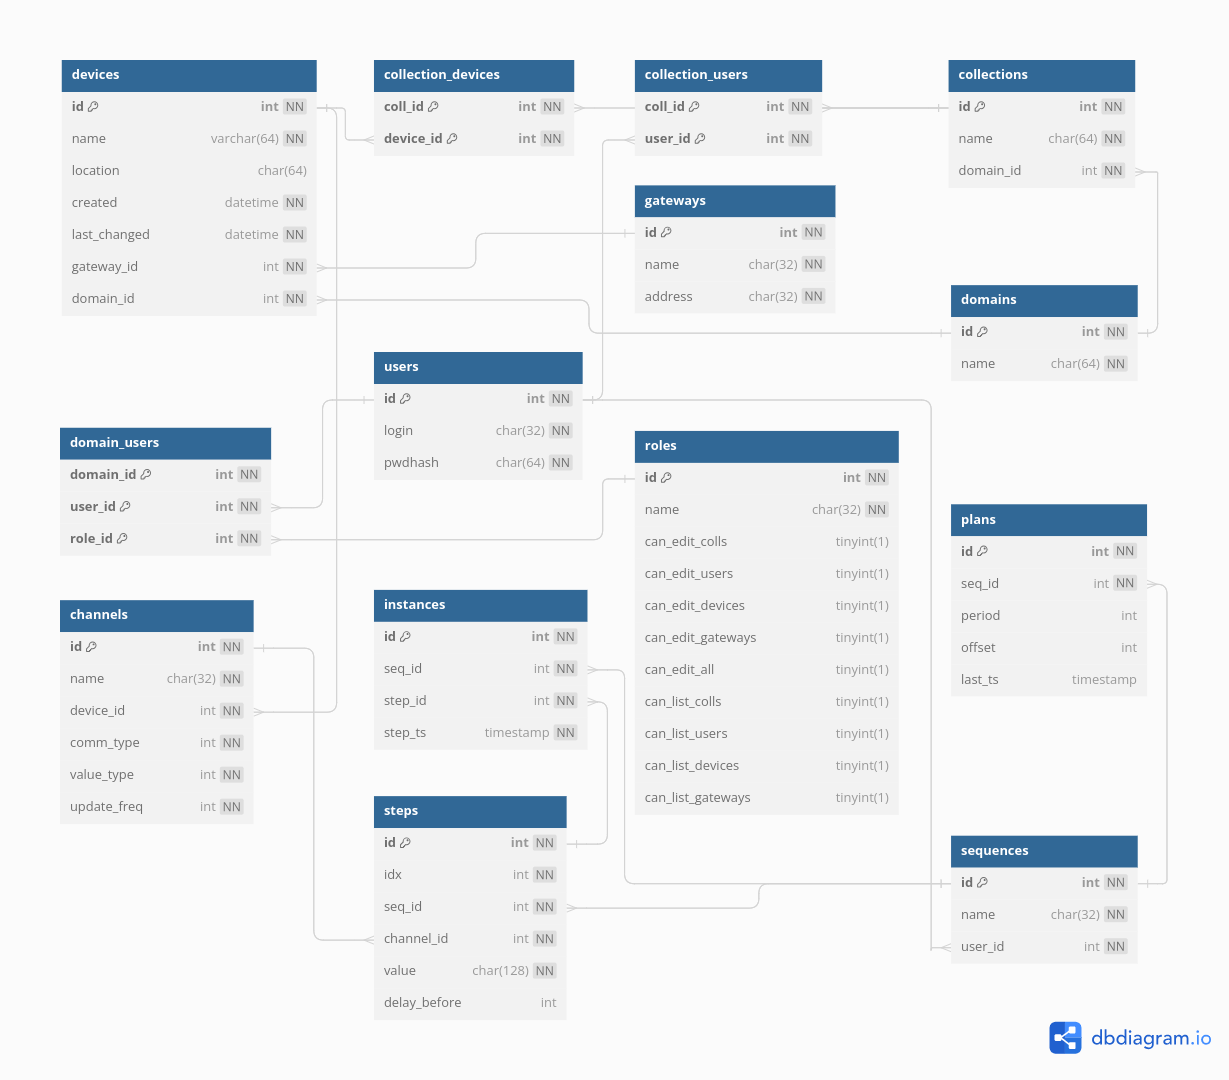
\includegraphics[width=1\textwidth]{images/database.png}
    \caption[Schéma tabulek databáze]{Schéma tabulek databáze \cite[\nopp Figure 1]{database_schema_generator}}
    \label{fig:my_label}
\end{figure}

\subsection{Tabulka zařízení}
Tabulka zařízení \emph{devices} obsahuje kromě sloupce s unikátním identifikátorem \emph{id} sloupce \emph{name} (jméno), \emph{location} (umístění), \emph{created} (datum vytvoření), \emph{last\_changed} (datum poslední změny), \emph{gateway\_id} (ID komunikační brány) a \emph{domain\_id} (ID domény). 

\emph{id} je číselná hodnota unikátní pro každý záznam, která slouží jako primární klíč této tabulky, můžeme tedy podle pouze této hodnoty jednoznačně nalézt hledaný záznam. \emph{location} je uživatelem zvolený popis umístění zařízení; tato hodnota slouží pouze k jednodušší identifikaci zařízení pro uživatele. Náhodným příkladem očekávané hodnoty by bylo například \emph{Obývací pokoj}. 

\emph{created} a \emph{last\_changed} jsou sloupce uchovávající časové hodnoty, v databázi MySQL se typ těchto polí označuje jako DATETIME. \emph{created} je nastavováno přímo databází při ukládání nového záznamu. \emph{last\_changed} by mělo být změněno při každé aktualizaci daného záznamu, sám SQL předpis to však nevyžaduje - režie změny je přenechána na systém, který vytváří SQL výraz pro změnu hodnot v záznamu.

\emph{gateway\_id} je hodnota, která referencuje sloupec \emph{id} v tabulce komunikačních bran. Databáze kontroluje existenci záznamu brány s touto hodnotou a neumožní zapsat do tabulky zařízení hodnotu, pro kterou neexistuje záznam v tabulce bran, a zároveň neumožní smazat záznam z tabulky bran, pokud je jeho \emph{id} zmíněno v záznamu v tabulce zařízení. Pro sloupec \emph{domain\_id} platí podobná pravidla, a to tedy že databáze kontroluje existenci záznamu s hodnotou \emph{id} v tabulce domén stejnou jako hodnotou \emph{domain\_id} v tabulce zařízení, a neumožní provést operaci, která by zapříčinila, že pro hodnotu ve sloupci \emph{domain\_id} v tabulce zařízení nebude existovat žádný záznam v tabulce domén, který by totožnou hodnotu měl uloženou ve svém sloupci \emph{id}.

Jelikož se bude tato závislost hodnoty sloupce X v tabulce A na hodnotách sloupce Y v tabulce B oběvovat častěji, zadefinujme pojem \emph{sloupec A.X} jako \emph{sloupec X z tabulky A}. Druhým zadefinovaným pojmem nechť je \emph{sloupec A.X referencuje B.Y}, znamenající \emph{hodnota v sloupci X.A musí být vždy naleznutelná alespoň v jednom záznamu ve sloupci Y.B a tato skutečnost je v každém výrazu upravujícím hodnoty těchto dvou tabulek kontrolována databází}. 

\subsection{Tabulka kanálů}
Tabulka kanálů \emph{channels} je složena ze záznamů pro jednotlivé komunikační kanály všech zařízení. Obsahuje sloupce \emph{id} (unikátní identifikátor), \emph{name} (název), \emph{device\_id} (ID zařízení), \emph{comm\_type} (typ komunikace), \emph{value\_type} (typ hodnoty) a \emph{update\_freq} (frekvence aktualizace).

Sloupec \emph{name} obsahuje krátký název informačního kanálu, například \emph{Vypínání} nebo \emph{Barva}. Hodnota je pouze pro lepší identifikaci kanálu pro uživatele. Sloupec \emph{device\_id} referencuje \emph{devices.id}, tedy zařízení, jehož kanálem je.

Hodnota \emph{comm\_type} určuje o jaký typ komunikace jde. Databáze podporuje počet typů omezený pouze maximální hodnotou datového typu int, nicméně tato aplikace určuje pouze 3 typy komunikace, a to následující:
\begin{description}
    \item[Jednosměrný kanál od zařízení k serveru,] který bude používán například v kanálu informujícím o aktuální teplotě od teploměru, tedy hodnota, která nemůže být nijak ovládána a je pouze oznamována serveru k zobrazení.
    \item[Jednosměrný kanál od serveru k zařízení,] který bude používán například u aktivace časovaného světla na chodbě, které nepodporuje možnost načtení aktuálního stavu, tedy kanál pro ovládání hodnoty, u které neumíme ověřit její stav.
    \item[Obousměrný kanál,] který bude používán například u zapínání chytrého osvětlení, které umí potvrdit aktuální stav serveru, a ten se tedy může dotázat a na základě výsledku například upravit zobrzení ovládacího prvku tohoto kanálu.
\end{description}
Typ komunikace je v databázi uložen číslem odpovídajícím jeho pozici v seznamu výše.

Sloupec \emph{value\_type} je používán k určení typu hodnot odesílaných v kanálu. Ačkoliv databáze umožňuje větší počet typů, aplikace využívá pouze následující:
\begin{itemize}
    \item{integer}, neboli číselnou hodnotu
    \item{rgb}, neboli trojici číselných hodnot 0-255, představující jednotlivé složky barvy popsané v RGB notaci.
    \item{bool}, neboli binární hodnotu true/false
    \item{string}, neboli posloupnost ASCII znaků v počtu 0-255 znaků.
\end{itemize}
Typ hodnot je v databázi uložen číslem odpovídajícím jeho pozici v seznamu výše.

Sloupec \emph{update\_freq} je délka intervalu, ve kterém se mají hodnoty daného kanálu měnit, v sekundách.

\subsection{Tabulka uživatelských účtů}

Tabulka uživatelských účtů \emph{users} uchovává záznamy, kde každý záznam odpovídá jednomu uživateli. Kromě \emph{id} (jednoznačného identifikátoru) obsahuje také sloupce \emph{login} (uživatelské jméno) a \emph{pwdhash} (výstup hashovací funkce sha256, jejímž vstupem bylo uživatelem zadané heslo). Sloupec \emph{login} je omezen 32 znaků a databáze automaticky kontroluje, aby hodnoty v něm zapsané byly unikátní. Sloupec \emph{pwdhash} je v databázi deklarovaný jako běžná posloupnost znaků char(64), použití funkce sha256 databáze neprovádí.

\subsection{Tabulka domén}

Tabulka domén \emph{domains} obsahuje údaje o doménách, neboli největších správních celcích v aplikaci. Skládá se ze sloupců \emph{id} (unikátního identifikátoru) a \emph{name} (názvu domény).

\subsection{Tabulka skupin}

Tabulka skupin \emph{collections} zaznamenává jednotlivé skupiny hráčů a zařízení. Kromě unikátního identifikátoru \emph{id} v ní najdeme také sloupce \emph{name} (jméno skupiny) a \emph{domain\_id} (ID domény). Hodnoty posledního zmíněného sloupce referencují sloupec \emph{domains.id}.

\subsection{Tabulka kroků}

Tabulka kroků \emph{steps} ukládá jednotlivé kroky sekvencí a jejich detaily. Používá k tomu sloupce \emph{id} (unikátní identifikátor), \emph{idx} (pořadí kroku v sekvenci), \emph{seq\_id} (ID sekvence), \emph{channel\_id} (ID kanálu), \emph{value} (obsah) a \emph{delay\_before} (pauza před provedením kroku).

Sloupec \emph{idx} obsahuje číslo značící pořadí kroku v sekvenci, které je využíváno pro rychlé hledání následujícího kroku. Sloupec \emph{seq\_id} obsahuje identifikátor sekvence, jejíž součástí je, a jeho data referencují sloupec \emph{sequences.id}. Data v sloupci \emph{channel\_id} referencují sloupec \emph{channels.id} v záznamu kanálu, ve kterém tento krok komunikuje, sloupec \emph{value} obsahuje data, která budou odeslána v předem zmíněném kanálu. Sloupec \emph{delay\_before} obsahuje čas v sekundách, který my měl být mezi odesláním předchozího kroku, případně spuštěním sekvence, a odesláním tohoto kroku.

\subsection{Tabulka sekvencí}

Tabulka sekvencí \emph{sequences} zaznamenává data týkající se posloupností kroků, které nazýváme sekvence, a obsahuje sloupce \emph{id} (unikátní identifikátor), \emph{name} (jméno sekvence) a \emph{user\_id} (ID uživatele, který sekvenci vytvořil). Hodnota sloupce \emph{user\_id} referencuje sloupec \emph{users.id}.

\subsection{Tabulka plánů}

Tabulka plánů \emph{plans} je složená ze záznamů, kde každý záznam odpovídá jednomu předem naplánovanému spuštění sekvence. Tento záznam je složený z hodnot \emph{id} (unikátní identifikátor), \emph{seq\_id} (ID plánované sekvence), \emph{period} (četnost spuštění plánu), \emph{offset} (zpoždění spuštění od základní jednotky četnosti) \emph{last\_ts} (časový údaj posledního spuštění plánu). Hodnota \emph{seq\_id} referencuje \emph{sequence.id}, 

\subsection{Tabulka instancí}

Tabulka instancí \emph{instances} obsahuje záznamy aktivně běžících sekvencí. Tyto záznam kromě vlastního unikátního identifikátoru \emph{id} uchovává odkaz na sekvenci pomocí sloupce \emph{seq\_id} (ID sekvence), který referencuje sloupec \emph{sequences.id}, odkaz na aktuálně plánovaný krok \emph{step\_id} (ID kroku) a časový údaj o čase, ve kterém by měl být tento krok proveden.

\section{Struktura MQTT komunikace}

Komunikaci pomocí protokolu MQTT nalezneme v aktuální verzi aplikace mezi MQTT zprostřed-kovatelem a webserverem, poté mezi MQTT zprostředkovatelem a jednotlivými komunikačními branami. Velkým problémem, který nastal v okamžiku rozhodnutí implementovat operační logiku serveru v jazyce PHP, navíc způsobem, který nezajišťuje, že bude tato část programu vždy běžící, byla ta skutečnost, že tato část aplikace tak nebude vždy dostupná pro odesílání a především příjem dat. Bylo tedy potřeba zajistit, aby zprávy, které odesílatel serveru odešle právě v momentě, kdy server nebude aktivně vykonávat PHP kód a tedy přijímat zprávy, byly serveru uchovány ve frontě, ze které by si je mohl při svém spuuštění načíst a tyto zprávy zpracovat.

Způsobů, jak takovou frontu naimplementovat, už je veřejně dostupných hned několik, pro naše účely se jako nejvhodnější volilo použít právě řešení implementující protokol MQTT neboli \emph{Message Queuing Telemetry Transport}. Tento protokol navrhuje strukturu, kde se uživatelé dělí na dva typy, a to zprostředovatelé (v originále zvané MQTT Broker) a klienty (MQTT Client). V dané síti je vždy jeden zprostředovatel, ostatní se poté připojují jako klienti. Komunikace probíhá vždy mezi zprostředovatelem a jedním z klientů, a to na systému postaveném na používání komunikačních témat (v originále Topic), ke kterým klient může požádat o zřízení odběru. Odebírat téma znamená dostat všechny zprávy zveřejněné v tématu. Zveřejnit zprávu v tématu (v originále Publish) může kterýkoliv uživatel.

Témata jsou uspořádány do struktury podobné adresářové cestě v běžných operačních systémech. Techologie MQTT také podporuje použití takzvaných divokých karet (Wildcards) při tvorbě požadavku k odběru. Díky tomu může klient požádat o odběr hned několika souvisejících témat zároveň.

Naše řešení využívá již hotové řešení jak MQTT zprostředkovatele, kterým je OCI obraz \emph{eclipse-mosquitto}, tak i MQTT klientů, kde byly použity dokonce dvě různá řešení kvůli rozdílům ve zvoleném jazyku implementace. Implementace Eclipse Mosquitto umožňuje přidání rozšiřujících pluginů, které přidávají nebo upravují funkcionalitu tohoto programu. V projektu jsem se rozhodl využít právě tuto implementaci mimo jiné i právě kvůli jednomu konkrétnímu pluginu, kterým je plugin \emph{Dynamic Security}. Ten rozšiřuje základní administraci uživatelů / klientů a omezování jejich přístupu k některým tématům, a díky němu lze publikováním konkrétní zprávy ve formmátu JSON na specifický kanál
upravovat účty, role a jejich přístupy bez nutnosti restartu zprostředkovatele.

Na straně webserveru je použita implementace v jazyce PHP s názvem \emph{php-mqtt/client}, dostupná pro instalaci pomocí nástroje Composer z repozitáře Packagist. Pro implementaci MQTT klienta v jazyce C/C++ jsem se rozhodl využít knihovnu libmosquitto.

\subsection{Přístupové účty}

Cílem tvorgy účtů je omezení přístupu jednotlivých MQTT klientů pouze k tématům, ke kterým by z návrhového hlediska mělo smysl přístup mít. Proto v této aplikaci vytvářím pro každého klienta vlastní účet. V MQTT zprostředkovateli máme nastavené dva trvalé statické účty a zbytek účtů generujeme dynamicky, jelikož v době tvorby kódu není známé, kolik klientů bude připojeno. 
Statickými účty jsou \emph{administrator} a \emph{webserver}. První zmíněný není používán žádnou komponentou v aplikaci, má absolutní práva a používá se pouze v případě manuálního zásahu administrátorem. Druhý zmíněný je samostatný účet pro webserver, který má statická práva pro odběr na kanály \emph{RegisteredGW} a \emph{Configs} a statická práva pro publikování na kanály \emph{GetConfigs} a \emph{\$CONTROL/dynamic-security/v1}.
Dynamické účty jsou generovány pro každou komunikační bránu, a to s uživatelským jménem dle předpisu \emph{GW/(označení brány)}. Označení brány je v aktuální verzi používaného návrhu komunikace MAC adresa zařízení, na kterém je software komunikační brány spuštěn. Tyto dynamicky vytvořené účty mají poté statická práva pro odběr na kanály \emph{RegisteredGW} a \emph{GetConfigs}, pro publikování na \emph{Configs}. Dále jsou těmto účtům přiděleny dynamická práva na témata vázaná ke konkrétní komunikační bráně.

\subsection{Statická témata}

V této sekci popisuji témata, která se používají po celou dobu běhu programu. Jsou to témata systémová, umožňující měnit nastavení a účty, nebo skupinová, ke kterým má práva k odběru nebo publikování více klientů.

\def\myprefix{}
\begin{enumnonum}[style=nextline]
    \item[GetConfigs]
    Toto téma je využíváno v procesu načítání konfiguračních souborů (dále KS) z připojených komunikačních bran. Webserver není obeznámen v případě připojení nové brány, proto tedy neposílá zádost o odeslání KS konkrétně jedné bráně, ale na takzvaný \emph{broadcast topic} - neboli do tématu, ke kterému mají registrovaný odběr všichni, nebo alespoň většina uživatelů. V okamžiku, kdy je do toho tématu publikována jakákoliv zpráva, všechny aktuálně připojené brány publikují svůj KS do tématu \emph{Configs}. Jelikož potřebujeme, aby nově připojené brány, které dosud němely vytvořený svůj účet, mohly také publikovat svůj KS a tak zajistit svou registraci, má právo k odebírání v tomto tématu i anonymní účet.
    \item[Configs]
    Právo k odebírání tohoto tématu má pouze uživatel \emph{webserver}. Funkce tématu \emph{Configs} je sbírat KS jednotlivých bran a doručit je webserveru, který s nimi můze dále pracovat. Je důležité, aby toto téma bylo ochráněno před neautorizovaným přístupem, jelikož právě v této části komunikace jsou přenášeny konfigurační data a osobní údaje. Je to jeden z největších argumentů pro použití pluginu \emph{Dynamic Security}, což sice zapříčíní složitější návrh a implementaci, ale zároveň zaručí, narozdíl od varianty, ve které by brány mohly přistupovat k systému pomocí \emph{anynomního účtu}, že si publikované zprávy v tomto tématu nemůže zobrazit žádná třetí strana. Kvůli možné probíhající první registraci nové brány mají k tomuto tématu právo publikovat i brány přistupující pomocí anonymního účtu.
    \item[RegisteredGW]
    Toto téma je používáno k notifikaci brány, že jí byl vytvořen přístupový účet a může tedy začít využívat autentizovaný přístup. Obsahem publikované zprávy je označení brány; stejné, jako brána používá ve svém uživatelském jméně. Právo k odběru tohoto tématu mají jak všechny účty bran, tak i anonymní účet. Pokud brána zachytí svůj identifikátor v publikované zprávě, je to pro ní značení, že má z anonymního přístupu přejít na spojení, ve kterém bude využívat svůj unikátní účet.
    \item[\$CONTROL/dynamic-security/v1]
    Témata s názvem začínajícím znakem \$ jsou dle konvence systémovými, často statistickými či jinak informačními tématy. Lze je přirovnat k primitivnímu konzolovému přístupu, kdy publikováním perfektně formulovaných zpráv lze docílit změn v nastavení. Na některá témata pro změnu publikuje přímo MQTT broker, lze z nich vyčíst záznamy událostí, jako lze u jiných platforem z \emph{log} souborů.
\end{enumnonum}

\subsection{Dynamicky vytvářená témata}

Pro doručování běžných zpráv jako je informace o aktuálním stavu komunikačního kanálu zařízení nebo odeslání nové hodnoty v tomto kanálu se využívají dynamicky generovaná témata pro každé zařízení a jeho kanály. Ty podléhají struktuře \emph{GW/(identifikátor brány)/(identifikátor zařízení)/(identifikátor kanálu)}. Identifikátorem zařízení i kanálu jsou v tomto kontextu jejich jména. Ačkoliv by se totiž na první pohled mohlo zdát, že je mnohem lepší i identifikaci využít pro tento účel vytvořené hodnoty sloupců \emph{id} v tabulce \emph{devices}, respektive \emph{channels}, tyto hodnoty zná pouze webserver, komunikační brána by podle nich tedy nebyla schopná identifikovat adresáta.
%---------------------------------------------------------------
\section{detailni popisovani kodu, problemu pri tvorbe, reseni}
%---------------------------------------------------------------


\subsubsection{jedna}
    aoinwroins
\subsubsection{dve}
    \paragraph{dve jedna}
    aa
    \paragraph{dve dve}
    aa
    \paragraph{dve tri}
    aa
\subsubsection{tri}
    aoinwroins


%---------------------------------------------------------------
\chapter{Testovani (2)}
%---------------------------------------------------------------

%---------------------------------------------------------------
\section{testovani}
%---------------------------------------------------------------
cíle                    3   
stávající řešení        2   6   7   cca 4
obecné                      2   3   cca 2
analýza                 18      9   cca 10
návrh                   20  10  10  cca 13
architektura            8   18      cca 10
realizace               10  8   12  cca 10
testování               6   8   1   cca 2